\chapter{Structured Peer-to-Peer Overlays}
\label{structured_p2p}
This chapter reviews structured overlays and introduces challenges and
proposed solutions regarding connectivity and performance.

\section{Background}
Structured P2P systems provide distributed look up services with guaranteed
search time with a lower bound of $O(\log N)$, in contrast to unstructured
systems, which rely on global knowledge/broadcasts, or stochastic techniques
such as random walks~\cite{unstructured_v_structured}.  Some examples of
structured systems can be found in~\cite{pastry, chord, symphony, kademlia,
can, brunet}.  In general, structured systems are able to make these guarantees
by self-organizing a structured topology, such as a 2D ring (pictured in
Figure~\ref{fig:ring_overlay}) or a hypercube.  Nodes joining an overlay
typically follow these steps:
\begin{enumerate}
\item generate or obtain a unique identification number (node ID) on the
order of 128-bits to 256-bits,
\item connect to a random address from a pre-shared well-known endpoints list,
\item become connected to at least one peer in the list (leaf connection),
\item find the peers closest in the address space to the selected node ID,
\item connect to nodes whose IDs are immediately smaller and / or larger than
itself (neighbor connections),
\item and finally connect to other nodes in the overlay that are not local in
the address space (shortcut connections).
\end{enumerate}

Each node must have a unique node ID; otherwise an address collisions can
prevent nodes from participating in the overlay and can potentially fragment
overlays, preventing them from working properly.  Having node IDs uniformly
distributed assists in providing improved routing in ring-based structured
overlays by requiring fewer shortcut connections than non-uniform distributions.
Each node can generate their own address if they use a cryptographically strong
random number generator.  Another approach for distributing node IDs relies upon
using a trusted third-party to generate and cryptographically sign node
IDs~\cite{secure_routing}.

A node must be connected to closest neighbors in the node ID address space;
optimizations for fault tolerance suggest that for ring topologies the amount
should be between 2 to $\log(N)$ on both sides.  In the case of overlay
disconnectivity especially when related to churn, when a peer does not know the
address of its immediate predecessor or successor and a message is routed
through it destined for them, depending on the message type, it may either be
locally consumed or thrown away, never arriving at its intended destination.
Having multiple neighbors assists in stabilizing the overlay structure when
experiencing churn, particularly when peers leave suddenly without warning.

Overlay shortcuts enable efficient routing in ring-based structured overlays.
The different shortcut selection methods include: maintaining large tables
without using connections and only verifying usability when routing
messages~\cite{pastry, kademlia}, maintaining a connection with a peer every
set distance in the P2P address space~\cite{chord}, or using locations drawn
from a harmonic distribution in the node address space~\cite{symphony}.

Most structured P2P overlays support decentralized storage/look-up of
information by mapping keys to specific node IDs in an overlay.  At a
minimum, the data is stored at the node ID either smaller or larger to the
data's node ID and for fault tolerance the data can be stored at other nodes.
This sort of mapping and data storage is called a distributed hash table (DHT).
DHTs provide the building blocks to form more complex distributed data stores
as presented in Past~\cite{past} and Kosha~\cite{kosha}.

There are two routing mechanisms for communication amongst peers in a
P2P overlay: iterative or recursive.  In iterative routing, the sender of a
packet will directly contact each successive member in a path querying it for
the next until arriving at the destination node, sending the packet directly to
the destination.  In recursive routing, messages are sent through the overlay
via forwarding from one peer to the next until arriving at the destination.
Compared to recursive routing, iterative can be implement more easily.  Though
iterative routing comes with considerable overhead, as each overlay query will
cause $\log(N)$ connections to form.  In addition, iterative routing makes NAT
traversal complicated, as it will require constant traversal mediation and need
to be made quickly; whereas recursive routing provides stable connections due
to a single NAT traversal during the connection phase.

\section{Network Address Translation Hampering P2P Systems}
As of 2010, the majority of the Internet is connected via Internet Protocol (IP)
version 4.  A limitation in this protocol is that there are only $2^{32}$
addresses (approximately 4 billion) available.  With the Earth's population of
over 8 billion and each individual potentially having multiple devices that
have Internet connectivity, the IPv4 limitation is becoming more and more
apparent.  To address this issue there have been two approaches:  1) the use of
network address translation (NAT) to enable many machines and devices to share
a single IP address but preventing bidirectional connection initiation, and 2)
IPv6 which supports $2^{128}$ addresses.  IPv6 does not necessarily imply
direct connectivity as there are no guarantees of NAT disappearing and outbound
only firewalls allowing incoming connections.

When a machine, \textit{A}, behind a typical NAT, \textit{B}, sends out a
packet to an Internet host, \textit{C}, the NAT device translates the packet so
that it appears it is coming from the NAT device making the NAT device a gateway.
When the the packet is sent from \textit{A} to \textit{C}, the source and
destination are listed as $IP:port$ pairs, where the source and destination are
$IP_A:Port_A$ and $IP_C:Port_C$, respectively.  \textit{A} forwards the packet
to \textit{B} who transforms the source from $IP_A:Port_A$ to $IP_B:Port_B$,
where $Port_A$ may or may not be equal to $Port_B$.  This creates a NAT mapping
so that incoming packets from $IP_C:Port_C$ to $IP_B:Port_B$ are translated and
forwarded to $IP_A:Port_A$.

There are a handful of recognized NAT devices as presented in~\cite{stun,
p2p_nats_rfc}.  The following list focuses on the more prevalent types:
\begin{itemize}
\item full cone - all requests from the same internal IP and port are mapped to
a static external IP and port, thus any external host can communicate with the
internal host once a mapping has been made,
\item restricted cone - like a full cone but requires that the internal host
has sent a message to the external host before the NAT will pass the packets,
\item port restricted cone - like a restricted cone but requires that the
internal host has sent the packet to the external hosts specific port before the
NAT will pass packets,
\item symmetric - each source and destination pair have no relation, thus only
a machine receiving a message from an internal host can send a message back.
\end{itemize}

Peers on cone NATs can easily be traversed so long as a third-party assists in
determining the port allocated by the NAT and as a medium for the peers to
exchange this information.  Peers behind symmetric NATs cannot easily
communicate with each other, since there is no relation between remote hosts
and ports and local ports.  Further complicating the matter is that there are
various types of symmetric NATs, having behaviors similar to full, restricted,
and port restricted cone NATs.  \cite{ice} describes methods to traverse
these NATs so long as there is a predictable pattern to port selection.  In
general, these approaches use UDP because of the lack of additional protocol
states, that require replay and ignoring reject methods that occur with the TCP
handshake,  though there is reasonable amount of work describing TCP NAT
traversal such as~\cite{tcp_nat}.  TCP NAT traversal is complicated by stateful
firewalls, or those that watch connections and connection attempts preventing
messages from closed TCP channels from passing through the NAT.  For situations
in which both peers are behind NATs and firewalls that prevent in bound
communication inhibiting NAT traversal, a third party can act as a relay
between the two, known as triangulation or TURN~\cite{turn} (traversal using
relay NAT).

\subsection{NAT Traversal in Structured Overlays}
Structured overlays rely on the principle that any peer can become directly
connected with any other peer in the system.  Thus in order to use structured
overlays on the Internet, they must either be run on publicly accessible
addresses or support NAT traversal.  Even in the case where there is NAT
traversal, occasionally there are Internet routing table breaks and two
peers who should be able to directly communicate cannot.

To date, there exists only one solution, Brunet~\cite{brunet}, supporting
decentralized UDP NAT traversal and limited relays.  To support UDP NAT
traversal, Brunet makes connection attempts bidirectional with peers exchange
all known IP addresses and ports, which it knows directly and from external
overlay nodes.  This enables the traversal of all forms of cone NATs, but
symmetric NATs require iterative rounds of traversal attempts and cannot be
traversed.  If two peers cannot connect, they exchange list of peers, if an
overlap exists, which is highly likely for peers adjacent on the overlay, they
will forward packets through it to each other other~\cite{hpdc08_1}.  This
approach focuses on forming a a correct structured ring not arbitrary two-hop
connections for high performance purposes.  This can be addressed by having
peers connect to each other's neighbor set proactively creating overlap, as
represented in Figure~\ref{fig:relay}.

In addition to exchanging overlap sets, peers also exchange some state of their
connections with the neighbors.  For example, the data shared could be
regarding node stability as measured by the age of a connection and proximity
as measured by ping latency to the neighbor.  When creating overlap or overlap
changes, peers review these metrics to decide which subset of the overlap to
use as a proxy leaving the remaining peers as reserves.

\subsection{Usefulness of Relays}
To determine the value in two-hop overlays as opposed to using the overlay in
restrictive NAT and firewall scenarios, this experiment uses an event-driven
simulator that reuses the code base of the prototype structured P2P VPN to
faithfully implement its functionality using event-driven simulated times to
emulate WAN latencies.  Pair-wise latency in this experiment is set using the
MIT King Data Set~\cite{king_data}, which consists of all-to-all latencies
among 1,740 distributed Internet hosts.  After starting the overlay and after
it has reached steady state, the simulator sends packets amongst all peers to
derive the average all-to-all latency and hop count for messaging in the
overlay.  In the low-latency relay model, each destination node forms a
connection to the source node's physically closest peer as determined via
latency (in a live system by application level ping).  Then this pathway is
used as a two-hop relay between source and node.  Only peers with two hops or
more are analyzed, as a single hop would only benefit under triangular
inequalities, which are not a consideration in this work.

Results are presented in Figure~\ref{fig:simulated_relays}. The network sizes
considered begin at 25 nodes because small networks of sizes 20 and under tend
to be fully connected in the underlying structured overlay.  It is not until
the network size expands past 100 and towards 200 nodes that relays become
significantly beneficial.  At 100 nodes, there is approximately a 54\%
performance increase, whereas at 200 there is an 87\% increase and it appears
to grow proportionately to the size of the pool, demonstrating the performance
advantage of two-hop autonomous relays.

In addition, the autonomous relays functionality were verified in a reference
implementation of a structured P2P VPN using a real system.  The environment
consists of PlanetLab as the public overlay and the Archer environment as the
VPN environment.  PlanetLab~\cite{planetlab} provides a set of over 500
distributed computing nodes all with public IP addresses.  Archer provides grid
computing to computer architecture researchers and consists of over 500 nodes
located at various academic sites.  To ensure that peers under study formed
two-hop connections, a firewall was instantiated preventing direct communication
between the two.  In tests, it was revealed that the overlay was always able to
self-configure a relay; the bandwidth and latency averages and deviations were
2245 Kbit/s $\pm$ 1080 and 58.1 ms $\pm$ 35.5, respectively.

\section{Using Structured Overlays for Direct Communication}
\label{direct_communication}
Applications like VPNs, games, media, and communication can benefit from using
an overlay for discovery and limited communication, though as communication
increases in frequency direct communication may be preferred.  In previous
work~\cite{wow}, the authors describe a method for transparently detecting this
behavior and creating direct links as a result.  In comparing a VPN built on
top of an overlay with a point-to-point direct approach, the VPN using the
overlay has significant overheads due to each IP packet traversing the overlay's
state machine prior to being sent to the VPN, established by
Table~\ref{tab:vpn_eval_comp}.  Thus for high bandwidth applications, this
approach does not scale and costs significant CPU utilization.

Two models in addition to the existing method of communication will be tested
to evaluate methods for obtaining high bandwidth using direct communication
links in overlay networks.  The two new approaches are:  1) use the structured
overlay to create and maintain links but placing the application between the
connection and the overlay stack so that the application has first access to
the data and 2) use the structured overlay to discover peers but the
application creates and manages its own links using the structured overlay to
coordinate these efforts.  %The proposed approaches are presented in
%Figure~\ref{fig:direct_communication}.

The first approach benefits from using existing components of the structured
overlay including link creation and maintenance though may still have overheads
due to packets needing to traverse both the application and overlays stack.
This can be addressed by creating a unique thread for processing packets in the
application as well as the overlay stacks.  Since the connections are shared,
this approach will require additional thread synchronization.

The second approach resides external from the structured overlay.  Th
application organizes communication links through the overlay but does not
communicate through it.  Though this is significantly more complicated than the
first solution, the application may be easier to code by reusing existing
overlay code.  Because each component has its own connections and communication
stacks, there is no need to handle synchronization between the overlay and
application.  Essentially, the application will have unfettered access to the
connections it has established.

Evaluation of these approaches will be performed using a VPN application as
described in Chapter~\ref{vpns}.

\section{Overlay-Aware TCP}
\label{tcp}
Communicating large amounts of data reliably and with good performance presents
an interesting challenge when performed through an overlay.  In an overlay,
peers are constantly joining and leaving a network, also known as churn.  During
churn, packets may be lost or misdirected, never arriving at their expected
destination.  Communication via an overlay may pass through many hops and
regardless of the communication protocol used, UDP or TCP, none are aware of
end to end behavior of the overlay focusing only on the point to point
communication between individual peers.  UDP complicates the matter by not
ensuring that communication between two peers is reliable, thus naive use of
UDP does not provide any information regarding the success of transferring a
packet between two peers.

To better understand the effects of overlays on reliable, high throughput
communication, a tool will be implemented to simulate such communication in
overlay environments with various amounts of churn to properly reflect both
dedicated and personal use of the environments.  In dedicated environments, the
behavior will most likely reflect that of the underlying Internet, though this
approach will benefit from proxies that the overlay can create when such outages
occur.  Personal use typically experiences many connections and disconnections,
though those peers that stay connected, tend to stay connected longer than
arriving peers.  The focus of this work will be to investigate existing TCP
solutions used in other networks and determine if there are other potential
solutions and evaluate them.

These results will then be used to implement an overlay-aware system for use in
a real P2P system that will be tested using the PlanetLab overlay.  Likewise with
the simulations, this work will confirm or help correct the modeling results and
provide insights on other potential solutions that may improve performance when
in a real system.

Most common TCP stacks implement a variety of components defined across
several works,\cite{tcp, tcp_congestion, tcp_hp, tcp_mss,
tcp_congestion_notification, tcp_sack}.  Implementing a system accurately
supporting these features could take a significant amount of time with little
research contributions.  There exist a few user space implementations already
support most of these features, such as lwIP~\cite{lwip} and and Userspace
network stack~\cite{unetstack}.  Initially, I will focus on creating a C\#
interface that allows deployment in the Brunet overlay.  If time allows, I will
create a native stack.

\section{Figures and Tables}

\begin{figure}[ht]
\centering
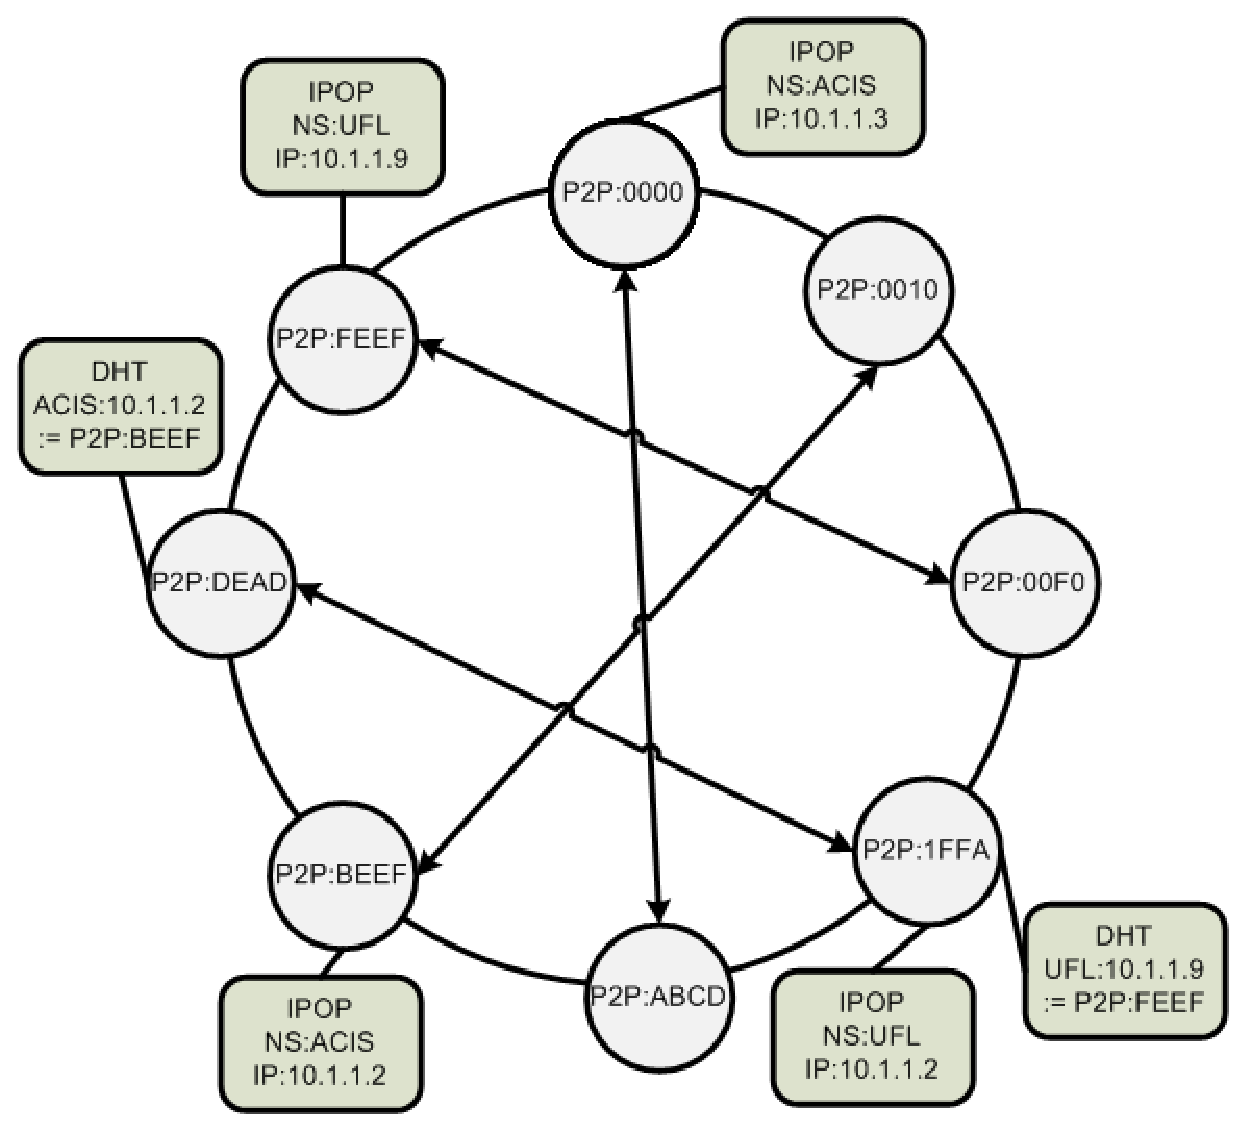
\epsfig{file=figs/ring.eps, width=4in}
\caption{1-D Ring Structured Overlay}
\label{fig:ring_overlay}
\end{figure}

\begin{figure}[ht]
\centering
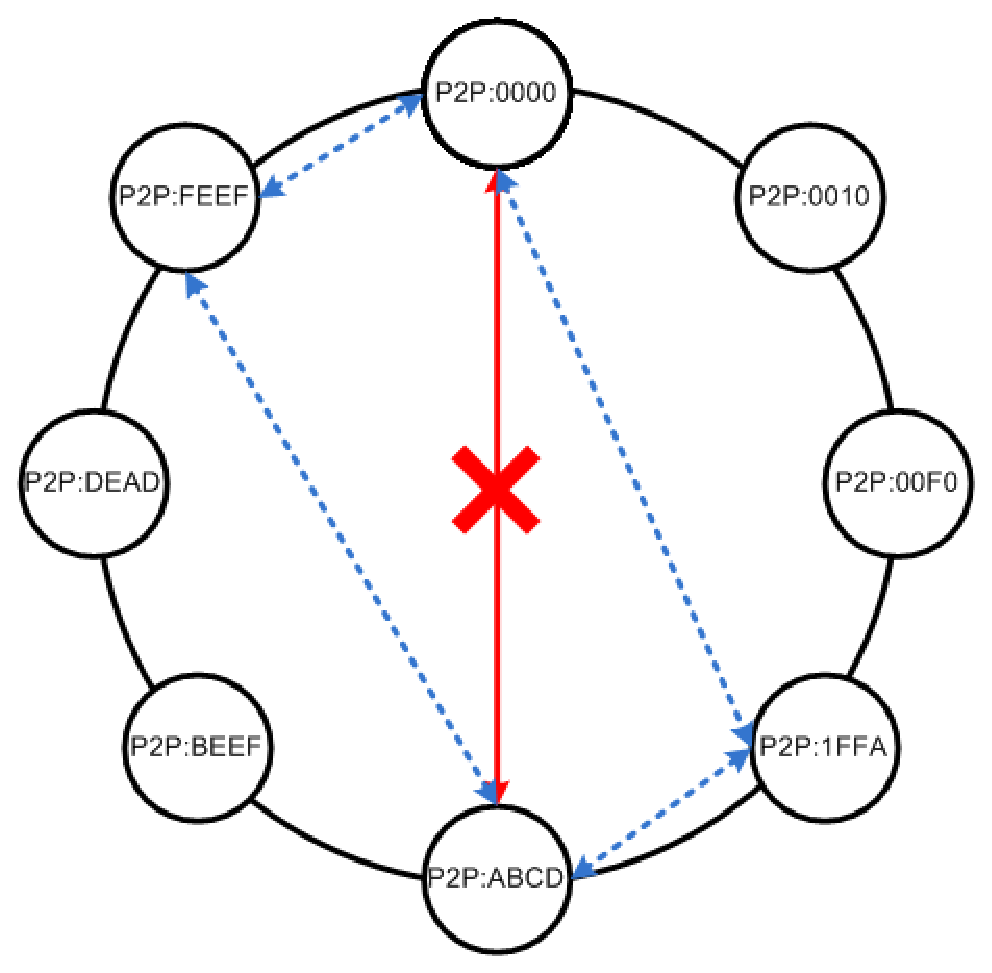
\epsfig{file=figs/relay.png.eps, width=4in}
\caption[Proactive relay creation]{Creating relays across the node address
space, when direct connectivity is not possible.  Two members, 0000 and ABCD, 
desire a direct connection but are unable to directly connect, perhaps due to
NATs or firewalls.  They exchange neighbor information through the overlay and
connect to one of each other's neighbors, creating an overlap.  The overlap
then becomes a relay path (represented by dashed lines), improving performance
over routing across the entire overlay.}
\label{fig:relay}
\end{figure}

\begin{figure}[ht]
\centering
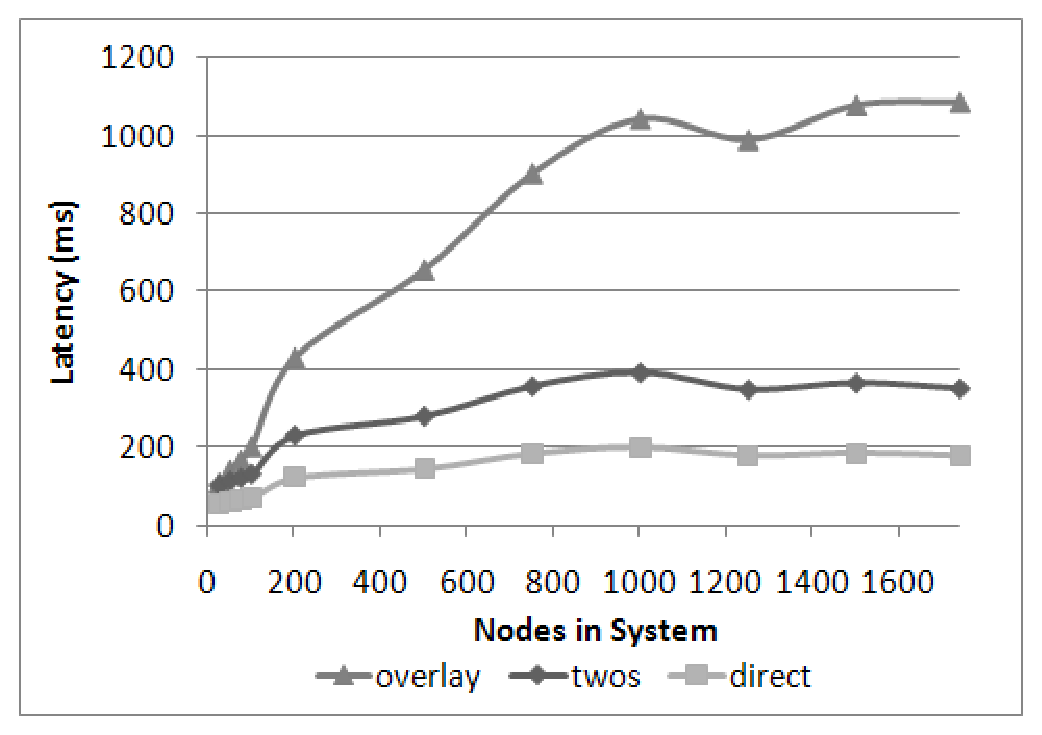
\epsfig{file=figs/relay_motivation.png.eps, width=4in}
\caption[Relay evaluation]{A comparison of the average all-to-all overlay
routing, two-hop relay, and direct connection latency in a Structured P2P
environment, Brunet, using the King data set.}
\label{fig:simulated_relays}
\end{figure}

%\begin{figure}[ht]
%\centering
%\caption{Direct communication models}
%\label{fig:direct_communication}
%\end{figure}

\begin{table}[ht]
\caption{VN Stack Comparison}
\label{tab:vpn_eval_comp}
\begin{tabular}{c||c|c|c}
& Latency (ms) & Bwidth (Mb/s) & Mem (KB) \\\hline
Host & 0.27 & 941 & n/a \\\hline
C & 0.34 & 738 & 998 \\\hline
C\# & 0.37 & 716 & 21500 \\\hline
IPOP & 0.52 & 284 & 38312 \\\hline
IPOP sec & 0.75 & 55 & 50976 \\\hline
\end{tabular}
\centering
\end{table}
